\documentclass{article}
\usepackage{amsmath}
\usepackage[utf8]{inputenc}
\usepackage{graphicx}
\usepackage{verbatim}
\usepackage{float}
\usepackage[makeroom]{cancel}
\usepackage[english]{babel}
\usepackage{textcomp}
\usepackage{gensymb}
\usepackage{color}
\usepackage{subcaption}
\usepackage{caption}
\usepackage{hyperref}
\usepackage{physics}
\usepackage{dsfont}
%\usepackage{amsfonts}
\usepackage{listings}
\usepackage{multicol}
\usepackage{units}

% From Eirik's .tex
\usepackage{epstopdf}
\usepackage{cite}
\usepackage{braket}
\usepackage{url}

\bibliographystyle{plain}

\usepackage{algorithmicx}
\usepackage{algorithm}% http://ctan.org/pkg/algorithms
\usepackage{algpseudocode}% http://ctan.org/pkg/algorithmicx

\usepackage[margin=1cm]{caption}
\usepackage[outer=1.2in,inner=1.2in]{geometry}
% For writing full-size pages
%\usepackage{geometry}
%\geometry{
%  left=5mm,
%  right=5mm,
%  top=5mm,
%  bottom=5mm,
%  heightrounded,
%}

% Finding overfull \hbox
\overfullrule=2cm

\lstset{language=IDL}
 %\lstset{alsolanguage=c++}
\lstset{basicstyle=\ttfamily\small}
 %\lstset{backgroundcolor=\color{white}}
\lstset{frame=single}
\lstset{stringstyle=\ttfamily}
\lstset{keywordstyle=\color{red}\bfseries}
\lstset{commentstyle=\itshape\color{blue}}
\lstset{showspaces=false}
\lstset{showstringspaces=false}
\lstset{showtabs=false}
\lstset{breaklines}
\lstset{aboveskip=20pt,belowskip=20pt}

\lstset{basicstyle=\footnotesize, basewidth=0.5em}
\lstdefinestyle{cl}{frame=none,basicstyle=\ttfamily\small}
\lstdefinestyle{pr}{frame=single,basicstyle=\ttfamily\small}
\lstdefinestyle{prt}{frame=none,basicstyle=\ttfamily\small}
% \lstinputlisting[language=Python]{filename}


\definecolor{codepurple}{rgb}{0.58,0,0.82}
\definecolor{backcolour}{rgb}{0.95,0.95,0.92}
\definecolor{dkgreen}{rgb}{0,0.6,0}
\definecolor{gray}{rgb}{0.5,0.5,0.5}
\definecolor{magenta}{rgb}{0.58,0,0.82}

\lstdefinestyle{pystyle}{
  language=Python,
  aboveskip=3mm,
  belowskip=3mm,
  columns=flexible,
  basicstyle={\small\ttfamily},
  backgroundcolor=\color{backcolour},
  commentstyle=\color{dkgreen},
  keywordstyle=\color{magenta},
  numberstyle=\tiny\color{gray},
  stringstyle=\color{codepurple},
  basicstyle=\footnotesize,
  breakatwhitespace=false,
  breaklines=true,
  captionpos=b,
  keepspaces=true,
  numbers=left,
  numbersep=5pt,
  showspaces=false,
  showstringspaces=false,
  showtabs=false,
  tabsize=2
}

%%%%%%%%%%%%%%%%%%%%%%%%%%%%%%%%
% Self made macros here yaaaaaay
\newcommand\answer[1]{\underline{\underline{#1}}}
\newcommand\pd[2]{\frac{\partial #1}{\partial #2}}
\newcommand\red[1]{\textcolor{red}{\textbf{#1}}}
\newcommand\numberthis{\addtocounter{equation}{1}\tag{\theequation}}
% Usage: \numberthis \label{name}
% Referencing: \eqref{name}

% Some matrices
\newcommand\smat[1]{\big(\begin{smallmatrix}#1\end{smallmatrix}\big)}
\newcommand\ppmat[1]{\begin{pmatrix}#1\end{pmatrix}}

%%%%%%%%%%%%%%%%%%%%%%%%%%%%%%%%%
% Eirik's self made macros
\newcommand{\s}{^{*}}
\newcommand{\V}[1]{\mathbf{#1}}
\newcommand{\husk}[1]{\color{red} #1 \color{black}}
\newcommand{\E}[1]{\cdot 10^{#1}}
\newcommand{\e}[1]{\ \text{#1}}
\newcommand{\tom}[1]{\big( #1 \big)}
\newcommand{\Tom}[1]{\Big( #1 \Big)}
\newcommand{\tomH}[1]{\big[ #1 \big] }
\newcommand{\TomH}[1]{\Big[ #1 \Big]}
\newcommand{\tomK}[1]{ \{ #1 \} }
\newcommand{\TomK}[1]{\Big\lbrace #1 \Big\rbrace}
\newcommand{\bigabs}[1]{\left| #1 \right|}

% Section labeling
\usepackage{titlesec}% http://ctan.org/pkg/titlesec
\renewcommand{\thesubsection}{\arabic{subsection}}


% Title/name/date
\title{FYS4150 - Project 2}
\author{Simen Nyhus Bastnes \& Eirik Ramsli Hauge}
\date{3. October 2016}

\begin{document}
\maketitle

\begin{abstract}
Wow dude, so this is like, so abstract dude. Have you ever had a dream that you, um, you had, your, you- you could, you’ll do, you- you wants, you, you could do so, you- you’ll do, you could- you, you want, you want them to do you so much you could do anything?
\end{abstract}
\subsection{Introduction}
In project 2, we aim to solve Schrödinger's equation for two electrons with and without a repulsive Coulomb interaction in a three-dimensional harmonic oscillator well. We start by reformulating the equation in a discretized form as an eigenvalue equation, which can be solved with Jacobi's method. \\\\

We can then compare our implementation Jacobi's method fares against ``smarter'' algorithms for solving eigenvalue equations. Finally, we will look at implementing unit-tests, in order to test that the various parts of our program does what it's intended to do.\\\\
\red{Should maybe be rewritten, or changed order, or add more, dunno}
\subsection{Theory}
\subsubsection{Schrödinger's equation}
In this project, we will assume that the electrons move in a three-dimensional harmonic oscillator potential, and repel each other via the static Coulomb interaction. By assuming spherical symmetry, the solution for the radial part of Schrödinger's equation for one electron reads
\begin{align*}
  -\frac{\hbar^2}{2m}\bigg(\frac{1}{r^2}\frac{d}{dr}r^2\frac{d}{dr} - \frac{l(l+1)}{r^2}\bigg)R(r) + V(r)R(r) = ER(r)\numberthis\label{eq:radial_schroedinger}
\end{align*}
For the rest of the project, we set the orbital momentum quantum number $l$ to zero. In our non-interacting case, the harmonic oscillator potential $V(r) = (1/2)kr^2$ with $k=m\omega^2$.\\\\We perform a substitution for $R(r) = (1/r)u(r)$, introduce a dimensionless variable $\rho = (1/\alpha)r$, where $\alpha$ is a constant with dimension length $\alpha = (\hbar^2/mk)^{1/4}$. Inserting this into the Scrödinger equation \eqref{eq:radial_schroedinger}, we get
\begin{align*}
-\frac{d^2}{d\rho^2}u(\rho) + \rho^2u(\rho) = \lambda u(\rho)\numberthis\label{eq:dimless_schroedinger}
\end{align*}
where $\lambda = (2m\alpha^2/\hbar^2)E$. Equation \eqref{eq:dimless_schroedinger} is the first equation we want to solve numerically, and we will later use that for $l=0$, the first eigenvalues $\lambda$ are $\lambda_0 = 3$, $\lambda_1 = 7$ and $\lambda_2 = 11$.\\\\
Starting our journey to write equation \eqref{eq:dimless_schroedinger} as an eigenvalue equation, we use the by now standard expression for the second derivative
\begin{align*}
  u'' = \frac{u(\rho+h)-2u(\rho)+u(\rho-h)}{h^2}+\mathcal{O}(h^2)
\end{align*}
where $h$ is our step length. We define minimum and maximum values for $\rho$, $\rho_{\text{min}} = 0$ and $\rho_{\text{max}}$, as we cannot set $\rho_{\text{max}} = \infty$. Next, we split this interval into $N$ number of mesh points, so that we can define the step length as
\begin{align*}
  h = \frac{\rho_N-\rho_0}{N}
\end{align*}
where $\rho_0 = \rho_{\text{min}}$ and $\rho_{\text{max}} =\rho_N$. This gives us an expression for $\rho$ at point $i$
\begin{align*}
  \rho_i = \rho_0 + ih\;\;\;\;\;\;\;\;\;i=1,2,\dots,N
\end{align*}
Now we can rewrite the second derivative as
\begin{align*}
  u_i'' = \frac{u_{i+1}-2u_i + u_{i-1}}{h^2}
\end{align*}
Using this, we can rewrite the dimensionless Schrödinger equation \eqref{eq:dimless_schroedinger} as a discretized equation.
\begin{align*}
  -\frac{u_{i+1}-2u_i+u_{i-1}}{h^2} + \rho_i^2u_i = -\frac{u_{i+1}-2u_i+u_{i-1}}{h^2} + V_iu_i = \lambda u_i 
\end{align*}
where $V_i = \rho_i^2$ is the harmonic oscillator potential. We can represent the left-hand side as a matrix multiplied by a vector $u$
\subsubsection*{Interacting case}
\begin{align*}
  V(\rho) = \omega_r^2\rho^2 + 1/\rho
\end{align*}
\subsubsection{Jacobi's method}
The aim of Jacobi's method is to use similarity transformation to make a $n \times n$ matrix into a diagonal $n \times n$ matrix with it's eigenvalues as the diagonal. We do this by starting with a matrix $\V{A}$ which is diagonally dominant \husk{REF TO WIKI!}. Within this matrix we find the largest element that is not on the diagonal, calling its indexes $k$ and $l$. The algorithm is as follows:
\begin{algorithm}[H]
\small
\caption{Maximum non-diagonal element}\label{alg:max_offdiag}
\begin{algorithmic}[1]
\State $max = 0.0$
\For{$i=0,\,n$}
\For{$j= i+1, \, n$}
\If{$|A[i][j]| > max$}
\State{$|A[i][j]| = max$}
\State{k = i}
\State{l = j}
\EndIf
\EndFor
\EndFor
\end{algorithmic}
\end{algorithm}
Now we want to rotate matrix $\V{A}$ such that the larges off-diagonal element becomes zero. This is done by using equation:
\begin{equation}
\V{B} = \V{S}^{\V{T}} \V{A} \V{S}
\label{eq:symtrans}
\end{equation}
Where $\V{S}$ is given as:
\begin{align*}
\ppmat{1 & 0 & \cdots & 0 & 0 & \cdots & 0 & 0 \\
	   0 & 1 & \cdots & 0 & 0 & \cdots & 0 & 0 \\
	   \vdots & \vdots & \ddots & \vdots & \vdots & \vdots & \vdots & \vdots \\
	   0 & 0 & \cdots & \cos \theta & 0 & \cdots & 0 & \sin \theta \\
	   0 & 0 & \cdots & 0 & 1 & \cdots & 0 & 0 \\
	   \vdots & \vdots & \vdots & \vdots & \vdots & \ddots & \vdots & \vdots \\
	   0 & 0 & \cdots & 0 & 0 & \cdots & 1 & 0 \\
	   0 & 0 & \cdots & -\sin \theta & 0 & \cdots & 0 & \cos \theta \\}
\end{align*}
With properties $\V{S}^{\V{T}} = \V{S}^{-1}$.
The positioning of $\cos \theta$ and $\sin \theta$ within the matrix is defined by the index of the largest off-digaonal element like this:
\begin{align*}
s_{kk} = s_{ll} = \cos\theta , \quad s_{kl} = -s_{lk} = \sin \theta, \quad s_{ii} = -s_{_ii} = 1 \quad i \neq k, \, i \neq l
\end{align*}
This is the same as performing a plane rotation around an angle $\theta$ in the Euclidean $n$-dimensional space. \\
For $\V{B}$ this gives us:
\begin{align*}
				b_{ii} 	&= a_{ii}, \ i \neq k, \ i \neq l \\
				b_{ik} 	&= a_{ik}\cos \theta - a_{il}\sin\theta,\ i \neq k, \ i \neq l \\
				b_{il} 	&= a_{il} \cos\theta + a_{ik}\sin\theta, \ i \neq k, \ i \neq l \\
				b_{kk} 	&= a_{kk}\cos^2\theta - 2a_{kl}\cos\theta \sin\theta + a_{ll}\sin^2\theta \\
				b_{ll} 	&= a_{ll}\cos^2\theta +2a_{kl}\cos\theta\sin\theta + a_{kk}\sin^2\theta \\
				b_{kl} 	&= (a_{kk} - a_{ll})\cos\theta \sin\theta +a_{kl}(\cos^2\theta - \sin^2\theta)
\end{align*}
Where $\theta$ is set as the angle that makes $b_{kl} = 0$. Each transformation can be proven to bring the matrix closer to the diagonal form. \husk{referer til forelesningsnotater}.  \\ \\
When all this is done, the old maxmium off-diagonal value will have become zero and a new one will have risen, but it will not be as large as the old one. We repeat our whole process until the maxmium value of all off-diagonal elements are below a certain threshold value. Ideally we would want them all to be zero, but very, very small values is good enough. \\
By looking at our expression for $b_kl = 0$ and defining
\begin{align*}
t = \tan\theta &= \frac{\sin\theta}{\cos\theta} \\
\tau = \cot 2\theta &= \frac{a_{ll} - a_{kk}}{2a_{kl}}
\intertext{We get:}
(a_{kk} - a_{ll})\cos\theta \sin\theta +a_{kl}(\cos^2\theta - \sin^2\theta) &= 0 \\
(a_{kk} - a_{ll})\cos^2\theta t + a_{kl}\cos^2\theta - a_{kl}\sin^2\theta &= 0 \\
(a_{kk} - a_{ll}) t + a_{kl} - a_{kl}\frac{\sin^2\theta}{\cos^2\theta} &= 0 \\
(a_{kk} - a_{ll}) t + a_{kl}(1-t^2) &= 0 \\
\frac{a_{kk} - a_{ll}}{a_{kl}} t &= t^2 -1 \\
-\tau t &= \frac{t^2-1}{2} \\
t^2 + 2 \tau t - 1 = 0, \quad &\Rightarrow \quad t = -\tau \pm \sqrt{1 + \tau^2}
\intertext{Cosine and sinus are easily found to be}
\cos \theta = \frac{1}{\sqrt{1 + t^2}}, \quad& \sin\theta = \cos\theta \cdot t
\end{align*} 
As we can see we can choose two different values for $t$. The one we want is the one that is the smallest. This is evident if we look at $b_{ik}$ and $b_{il}$. Hopefully these values will quickly reach values near zero and  we want to keep them there. To do this we want $\cos \theta$ to go to 1 and $\sin \theta$ to go to 0 simultaniously. By always choosing the lowest $t$-value we choose the lowest possible angle and therefore we will minimize the changes to the non-diagonal elements in the matrix. Except for $b_{kl}$ which is always set to zero. \\ \\

To fully grasp the idea of this method we have imagined it as this: \\
Let us pretend that you have ten bars in front of you. These bars can be pushed down, but as you push down one, the others will be affected also. We want to push all the bars as far down as possible, and if you push down the highest bar, the others can't reach it's height, but they are free to go up and down. Then all you have to do is push down one bar (find the maximum non-diagonal element and rotate the matrix) see how the other bars react (view the matrix after rotation), locate the bar that is now the highest and push that one down. As you do this, gradually all the bars will come under a certain height, even though they may not be completely pushed down. When you are satisfied with the shortness of the tallest bar, your job is done and we have found our diagonal matrix with eigenvalues. \\ \\
\husk{Jacobi's algorithm here?}
\subsection{Experimental?}
\subsection{Results}
\husk{We need to make graphs of $|\Psi(\rho)|^2$ for $\lambda_1$ etc.}
\subsubsection{Unit test}
From the three implemented unit tests all three passed.
\subsection{Discussion}
\begin{figure}[H]
  \centering
  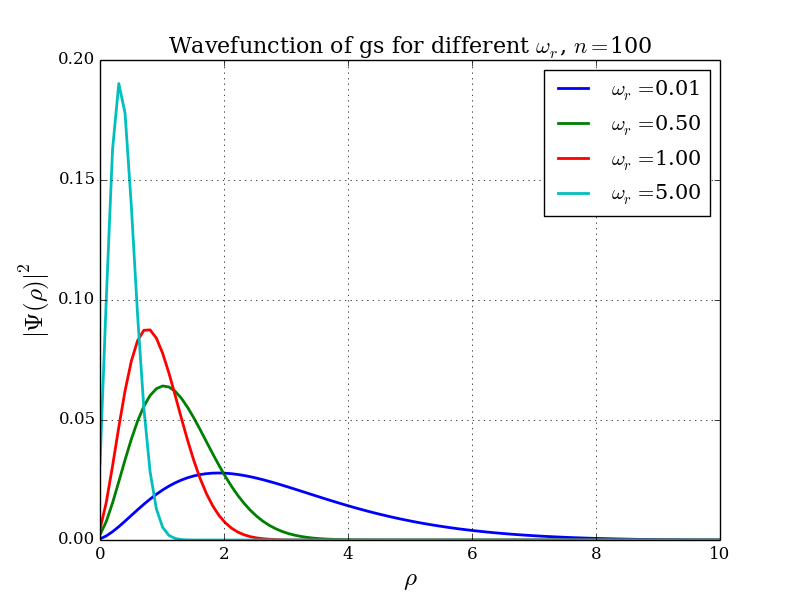
\includegraphics[scale=0.5]{../figures/eigvec_interact_n100.png}
  \caption{Plot of the eigenvectors for the interacting case for $n=100$}
  \label{fig:eigvec100}
\end{figure}
\subsection{Conclusion}
\bibliography{references}
\end{document}
